\documentclass[12pt, a4paper]{article}

\usepackage[hmargin=2.5cm, vmargin=2cm]{geometry}
\usepackage{amsthm, amssymb, mathtools, yhmath, graphicx}
\usepackage{fontspec, type1cm, titlesec, titling, fancyhdr, tabularx}
\usepackage{color, unicode-math, float, siunitx}
\usepackage{subcaption}
\usepackage[siunitx]{circuitikz}

\usepackage[CheckSingle, CJKmath]{xeCJK}
\usepackage{CJKulem}
\usepackage{enumitem}
%\setCJKmainfont[BoldFont=cwTex Q Hei]{cwTex Q Ming}
%\setCJKsansfont[BoldFont=cwTex Q Hei]{cwTex Q Ming}
%\setCJKmonofont[BoldFont=cwTex Q Hei]{cwTex Q Ming}
\setCJKmainfont[BoldFont=cwTeX Q Hei]{cwTeX Q Ming}

\def\normalsize{\fontsize{12}{18}\selectfont}
\def\large{\fontsize{14}{21}\selectfont}
\def\Large{\fontsize{16}{24}\selectfont}
\def\LARGE{\fontsize{18}{27}\selectfont}
\def\huge{\fontsize{20}{30}\selectfont}

%\titleformat{\section}{\bf\Large}{\arabic{section}}{24pt}{}
%\titleformat{\subsection}{\large}{\arabic{subsection}.}{12pt}{}
%\titlespacing*{\subsection}{0pt}{0pt}{1.5ex}

\parindent=24pt

\DeclarePairedDelimiter{\abs}{\lvert}{\rvert}
\DeclarePairedDelimiter{\norm}{\lVert}{\rVert}
\DeclarePairedDelimiter{\inpd}{\langle}{\rangle}
\DeclarePairedDelimiter{\ceil}{\lceil}{\rceil}
\DeclarePairedDelimiter{\floor}{\lfloor}{\rfloor}

\newcommand{\samp}{\si{\ampere}}
\newcommand{\smia}{\si{\milli\ampere}}
\newcommand{\svol}{\si{\volt}}
\newcommand{\skv}{\si{\kilo\volt}}
\newcommand{\sohm}{\si{\ohm}}
\newcommand{\skom}{\si{\kilo\ohm}}
\newcommand{\sdb}{\si{\decibel}}
\newcommand{\shz}{\si{\hertz}}
\newcommand{\img}{\mathrm{i}}
\newcommand{\dD}{\mathrm{d}}
\newcommand{\iD}{\:\mathrm{d}}
\newcommand{\Ans}{{\\ \bf Ans:} \\}

\usetikzlibrary{calc, arrows}

\begin{document}

\section{2.27}
The circuit in Fig below can be can be consider to be an extension of the circuit in Fig. 2.8

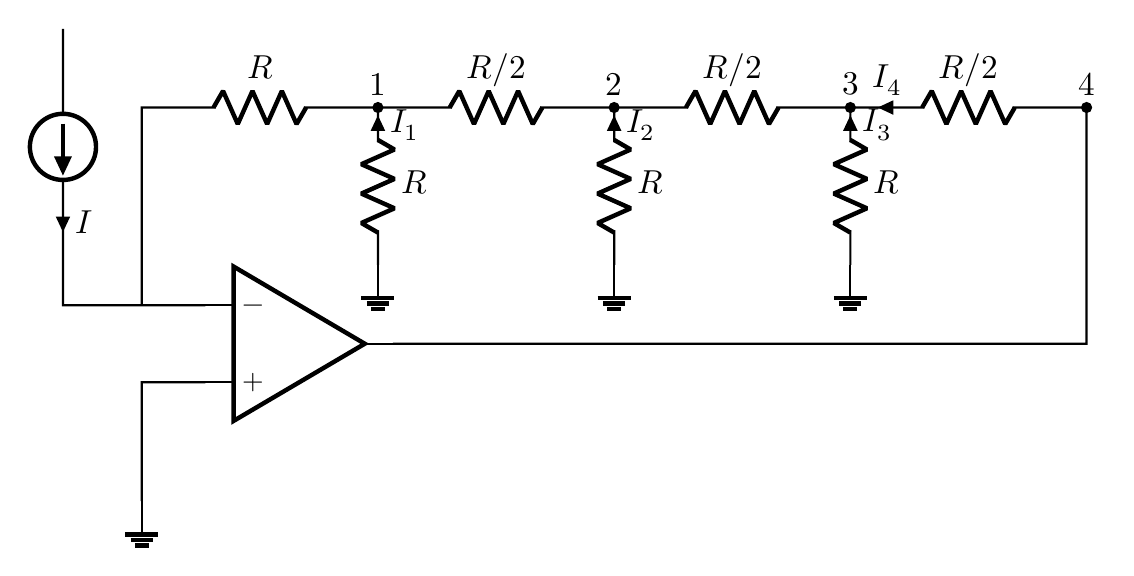
\begin{tikzpicture}[american voltages, american currents]
	\draw[color=black, thick]
  (0, 6) to [I=$I$] (0, 3) 
  %(0, 3) to [short] (3, 3)
  (3, 2) node[op amp](op) {}
  (op.-) -| (0, 3)
  (op.-) -| (1, 5) to[R, l=$R$, -*] (4, 5) to[R, l=$R/2$ ,-*] (7, 5) to[R, l=$R/2$, -*] (10, 5) to[R, l=$R/2$, i<=$I_4$, -*] (13, 5)
  (op.out) -| (13, 5)
  (4, 5) to [R, l=$R$, i<=$I_1$] (4, 3) node[ground]{}
  (7, 5) to [R, l=$R$, i<=$I_2$] (7, 3) node[ground]{}
  (10, 5) to [R, l=$R$, i<=$I_3$] (10, 3) node[ground]{}
  (op.+) -| (1, 0) node[ground]{}
  (4, 5) node[above]{$1$}
  (7, 5) node[above]{$2$}
  (10, 5) node[above]{$3$}
  (13, 5) node[above]{$4$}
	;
\end{tikzpicture}

\begin{enumerate}[label=(\alph*)]
  \item Find the resistance looking into node 1, 2, 3, 4.\\
    \Ans
    \begin{align*}
      R_1 &= R\\
      R_2 &= (R_1 || R) + R / 2 = R\\
      R_3 &= (R_2 || R) + R / 2 = R\\
      R_4 &= (R_3 || R) + R / 2 = R\\
    \end{align*}
  \item Find the currents $I_1, I_2, I_3, I_4$, in terms of $I$\\
    \Ans
    \begin{align*}
      I_1 &= IR / R = I\\
      I_2 &= ((I+I_1) (R/2) + IR) / R= 2I\\
      I_3 &= (4IR/2 + 2IR)/R = 4I \\
      I_4 &= -(4I + 4I) = -8I 
    \end{align*}
  \item Find the voltages at node 1, 2, 3, 4.\\
    \Ans
    \begin{align*}
      V_1 &= -IR               \\
      V_2 &= V_1 + 2IR/2 = -2IR\\
      V_3 &= V_2 + 4IR/2 = -4IR\\
      V_4 &= V_3 + 8IR/2 = -8IR
    \end{align*}
\end{enumerate}

\section{2.28}
The circuit below utilizes an ideal op amp.\\
\begin{figure}[H]
\centering
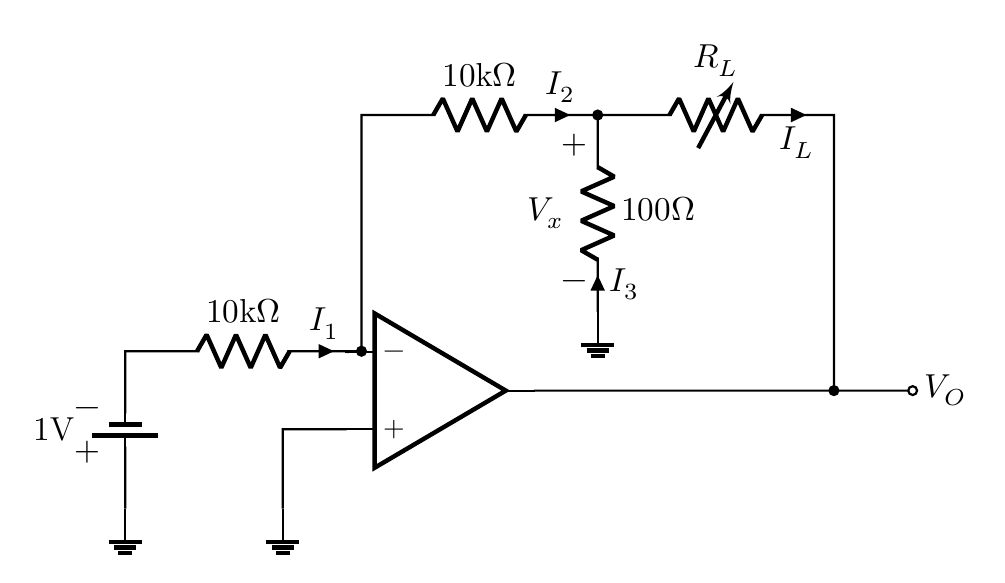
\begin{tikzpicture}[american voltages, american currents]
	\draw[color=black, thick]
  (0, 0) node[ground]{} to [battery1=$1\si{\volt}$] (0, 2) to [R, l=$10\si{\kilo\ohm}$, i>=$I_1$, -*] (3, 2) -- (3, 5) to [R, l=$10\si{\kilo\ohm}$, i>=$I_2$, -*] (6, 5) (6, 5) to [vR, l=$R_L$, i_>=$I_L$] (9, 5) -| (9, 1.5)
  (4, 1.5) node[op amp](op) {}
  (op.-) to [short] (3, 2)
  (2, 0) node[ground]{} |- (op.+)
  (op.out) to [short, -*] (9, 1.5) to [short, -o] (10, 1.5) node[right]{$V_O$}
  (6, 5) to [R, l=$100\si{\ohm}$, v=$V_x$, i^<=$I_3$] (6, 2.5) node[ground]{}
	;
\end{tikzpicture}
\end{figure}
\begin{enumerate}[label=(\alph*)]
  \item Find $I_1, I_2, I_3, V_x$
    \Ans 
    \begin{align*}
      I_1 &= 1\si{\volt} / 10\si{\kilo\ohm} = 0.1\si{\milli\ampere}\\
      I_2 &= I_1 = 0.1\si{\milli\ampere}\\
      V_x &= 0 - (0.1\si{\milli\ampere})(10\si{\kilo\ohm}) = -1 \si{\volt}\\
      I_3 &= 1 / 100\si{\ohm} = 10\si{\milli\ampere}
    \end{align*}
  \item If $V_O$ is not to be lower than $-13\si{\volt}$, find the maximum allowed value of $R_L$
    \Ans 
    \begin{align*}
      V_O &= V_x + R_L I_L = V_x + R_L (I_2 + I_3)\\
          &= - 1\si{\volt} - (10.1 \smia) R_L
    \end{align*}
    so
    \[
      R_L \leq 12\svol / 10.1 \smia \approx 1.19
    \]
  \item If $R_L$ is varied in the range $100 \sohm$ to $1 \si{\kilo\ohm}$, what is the corresponding change in $I_L$ and in $V_O$?
    \Ans
    $I_L$ would not change\\
    \[
      V_O \rvert_{R_L = 100 \sohm} = -2.01 \svol, V_O \rvert_{R_L = 1\skom} = -11.1\svol
    \]
\end{enumerate}


\section{2.37}
Figure P2.37 shows a circuit for a digital-to-analog converter. The circuit accepts a 4-bit input binary word $a_3a_2a_1a_0$ where $a_i \in \{0, 1\}$. Each of the bits of the input word controls the correspondingly numbered switch. For instance, if $a_2$ is 0 then switch $S_2$ connects the $20 \skom$ resistor to ground, while if $a_2$ is $1$ then $S_2$ connects the $20 \skom$ resistor to the $+5\svol$ power supply.
Show that $v_O$ is given by
\[
  v_O = - \frac{R_f}{16} \sum_{i=0}^{3} 2^i a_i
\]
where $R_f$ is in kiloohms. Find the value of $R_f$ so that $v_O$ ranges from $0$ to $-12\svol$.\\

\begin{circuitikz}[
    arw/.style={->, thick, shorten <=2pt, shorten >=2pt},
    >=triangle 45,
  ]
  \draw[color=black, thick][american voltages, american currents]
  (0, 0) node[spdt, xscale=-1, label={[label distance=.4cm]above:$S_0$}] (s1) {}
  (0, 3) node[spdt, xscale=-1, label={[label distance=.4cm]above:$S_1$}] (s2) {}
  (0, 6) node[spdt, xscale=-1, label={[label distance=.4cm]above:$S_2$}] (s3) {}
  (0, 9) node[spdt, xscale=-1, label={[label distance=.4cm]above:$S_3$}] (s4) {}
  (s4.in) to[R, l=$10\skom$] ++(3, 0) to [short] ($ (s1.in)+(3, 0) $)
  (s3.in) to[R, l=$20\skom$, -*] ++(3, 0) node(p1){}
  ($ (p1)+(2.5,-1.5) $) node[op amp](op){}
  (s2.in) to[R, l=$40\skom$, -*] ++(3, 0)
  (s1.in) to[R, l=$80\skom$] ++(3, 0)
  ($ (p1)+(0,-1) $) to[short, *-*, i={\color{red}$I_1$}] ++(1, 0) to[short] ++(0, 1) to[R, l=$R_f$] ++(3, 0) to[short, -*] ++(0, -1.5) to[short, -o] ++(.5, 0)node(p2){} to[open, v=$v_O$] ++(0, -2) node[ground]{}
  (op.-) to[short] ($ (p1)+(1,-1) $) 
  (op.+) node[ground]{}
  (op.out) to[short] (p2)
  ;
  \draw[arw]
  (s1.out 1) to ++(-1, 0) node[left]{$+5\svol$};
  \draw[arw]
  (s2.out 1) to ++(-1, 0) node[left]{$+5\svol$};
  \draw[arw]
  (s3.out 1) to ++(-1, 0) node[left]{$+5\svol$};
  \draw[arw]
  (s4.out 1) to ++(-1, 0) node[left]{$+5\svol$};
  \draw
  (s1.out 2) node[ground] {}
  (s2.out 2) node[ground] {}
  (s3.out 2) node[ground] {}
  (s4.out 2) node[ground] {}
  ;
\end{circuitikz}
\Ans
Note that 
\[
  I_1 = \sum_{i=0}^{3} a_i (5\svol) / (10 \cdot 2^{(3-i)} \skom) = \sum_{i=0}^{3} a_i / 2^{(4-i)} (\smia)
\]
so
\[
  v_O = 0 - R_f I_1 = - R_f \sum_{i=0}^{3} a_i 2^i / 16.
\]
If $v_O$ ranges from \SI{0}{\volt} to \SI{12}{\volt}, then
\[
  v_O = -\frac{R_f}{16} \sum_{i=0}^{3} a_i 2^i \Rightarrow
  0 \ge v_O \ge -\frac{15}{16}R_f.
\]
So $R_f = 12.8\skom$.

\section{2.51}
Figure shows a circuit that provides an output voltage $v_o$ whose value can be varied by turning the wiper of the 100\skom potentiometer. Find the range over which $v_o$ can be varied. If the potentiometer is a "20-turn" device, find the change in $v_o$ corresponding to each turn of the pot.

\begin{circuitikz}
	\draw[color=black, thick][american voltages, american currents]
  (0, 9) to [R, l=$20\skom$] (0, 6) to [pR, l_=$100\skom$, n=pot] (0, 3) to [R, l=$20\skom$] (0, 0)
  (4, 5) node[op amp](op) {}
  (0, 0) to [short, -*] (3, 0) -| (op.down)
  (op.up) |- (3, 9) to [short, *-] (0, 9)
  (op.+) to[short, -*] ++(-1, 0) node[label={\color{red}$v_1$}]{} to[short] (pot.wiper)
  (op.out) to [short, -*] ++(.5, 0) to [short, -o] ++(.5, 0) node[right] {$v_O$}
  (op.out)+(.5, 0) |- ++(-3, 2) |- (op.-)
	;
  \draw (3, 0) node[below] {$-15\svol$};
  \draw (3, 9) node[above] {$+15 \svol$};

\end{circuitikz}
\Ans
We have
\begin{align*}
  v_O &= v_1 \\
  v_{1, \text{max}} &= (15\svol) \frac{100 + 20}{100 + 20 + 20} + (-15\svol) \frac{20}{100 + 20 + 20} \approx 10.7\svol \\
  v_{1, \text{min}} &= - v_{1, \text{max}}
\end{align*}
And so the voltage change each turn is $(v_{1, \text{max}} - v_{1, \text{min}}) / 20 \approx 1.07$.
\section{2.63}

For an instrumentation amplifier of the type shown in Fig 2.20(b), a designer proposes to make $R_2 = R_3 = R_4 = 100\skom$ and $2R_1 = 10\skom$. For ideal components, what difference-mode gain, common-mode gain, and CMRR result? Reevaluate the worst-case values for these for the situation in which all resistors are specified as $\pm 1\%$ units. Repeat the latter analysis for the case in which $2R_1$ is reduced to $1 \skom$. What do you conclude about the importance of the relative difference gains of the first and second stages?
\Ans
\begin{circuitikz}
	\draw[color=black, thick][american voltages, american currents]
  (2, .5) node[op amp](op2) {}
  (2, 5.5) node[op amp, yscale=-1](op1) {}
  (8, 3) node[op amp](op3) {}
  (op1.+) to[short, -o] ++(-2, 0) node[left]{$v_{I1}$}
  (op2.+) to[short, -o] ++(-2, 0) node[left]{$v_{I2}$}
  (op2.-) -| ++(-1, .8) node[](v2){}
  (op1.-) -| ++(-1, -.8) node[](v1){}
  (op1.out) to[short, -*] ++(.5, 0) node[](v3){} to[short] ++ (0, -1.3) to [R, l=$R_{21}$] (v1) to [R, l=$2R_{1}$] (v2)
  (op2.out) to[short, -*] ++(.5, 0) node[](v4){} to[short] ++ (0, 1.3) to [R, l_=$R_{22}$] (v2)
  (v3) to[short] ++(0.5, 0) -| ++(.5, -2) to [R, l=$R_{31}$] (op3.-) -- ++(0, 1) to [R, l=$R_{41}$] ++(3, 0) to[short] ++(0, -1.5)node[](v5){} to[short, *-o] ++(1, 0) to[open, v^=$v_O$] ++(0, -3) node[ground]{}
  (v4) to[short] ++(0.5, 0) -| ++(.5, 2) to [R, l_=$R_{32}$, -*] (op3.+) to [R, l=$R_{42}$] ++(0, -2.5) node[ground]{}
  (op3.out) to[short] (v5)
  ;
  \draw[dashed] (-.5, -.5) rectangle ($ (v3) + (.5, 1) $);
  \draw[dashed] ($(v4) + (.7, -1) $) rectangle ($ (v5) + (.5, 2.5) $);
  \draw (-1.8, 3) node[text width=1.5]{First stage};
  \draw (7.5, 5.8) node[]{Second stage};
\end{circuitikz}

If the resistor are ideal, the circuit is same as the textbook circuit, So as in textbook, we have
\begin{align*}
  A_{cm} &= 0\\
  A_{d} &= \frac{R_4}{R_3} \left(1 + \frac{R_2}{R_1} \right)\\
  &= 1 \cdot (1 + 100 / 5) = 21
\end{align*}
CMRR is then $20\log\left(\frac{A_{Id}}{A_{Icm}}\right) = \infty$.\\

Now if all resistors are specified as $\pm 1\%$ units. First consider the first stage gain, the common-mode gain would be maximize by letting $R_{31} = R_{42} = 101\skom, R_{32} = R_{41} = 99\skom$, and
\[ A_{cm} = \frac{R_{42}}{R_{32}+R_{42}}
  \left( 1 - \frac{R_{41}R_{32}}{R_{31}R_{42}} \right)
  \approx \SI{1.98e-2}{\volt/\volt}. \]
  The difference-mode gain wouldn't be affect too much by the resistor bias. \\
At the first stage. In the worse case, the minimize difference-mode gain by let $2R_1 = 10.1\skom, R_2 = 99\skom$.
\[ A_{d} = \frac{2R_2 + 2R_1}{2R_1}\frac{1}{R_{31}}\frac{1}{R_{32}+R_{42}}
  (R_{31}R_{42}+2R_{41}R_{42}+R_{32}R_{41}) \approx \SI{20.4}{\volt/\volt}.
\]
  And the common-mode gain is $0$ in every situation. So the overall CMRR is $20\log\left(\frac{A_{d}}{A_{cm}}\right) \approx 60.26\sdb$. \\
If $2R_1 = 1\skom$, then By similar calculation, $A_{d} \approx \SI{201}{\volt/\volt}$.  The first stage dominates the difference-mode gain.  And the common-mode gain doesn't change. So CMRR is
$20\log\left(\frac{A_{Id}}{A_{Icm}}\right) \approx 80.13\sdb$.

\section{2.65}
The circuit shown in Fig is intended to supply a voltage to floating loads (those for which both terminals are ungrounded) while making possible use of available power supply.

\begin{circuitikz}
	\draw[color=black, thick][american voltages, american currents]
  (6, 0.5) node[op amp](op1){}
  (6, 3.5) node[op amp](op2){}
  (0, 0) node[ground]{} to [R, l=$10\skom$] (op1.+)
  (0, 2) to[short, o-*] ++(1, 0) -- ++(0, -1) to [R, l=$10\skom$, -*] (op1.-) -- ++(0, 1) to [R, l=$30\skom$] ++(3, 0) to [short] ++(0, -1.5) node(p1){} to[short, -o] ++(0.5, 0) node[right](C){C}
  (op1.out) to [short, -*] (p1)
  (1, 2) -- ++(0, 1) to [R, l=$10\skom$] (op2.+)
  (0, 4) node[ground]{} to [R, l=$10\skom$, -*] (op2.-) -- ++(0, 1) to[R, l=$20\skom$] ++ (3, 0) to [short] ++(0, -1.5) node(p2){} to [short, -o] ++(.5, 0) node[right](B){B}
  (op2.out) to [short, -*] (p2)
  (0, 2) to [open, v=$v_I$] (0, 0)
  (B) to [open, v^=$v_O$] (C)
	;
\end{circuitikz}

\begin{enumerate}[label=(\alph*)]
  \item Assuming ideal op amps, sketch the voltage waveforms at nodes B and C for a $1\svol$ peak-to-peak sine wave applied at A. Also sketch $v_O$
  \Ans
  \begin{figure}[H]
    \centering
    \includegraphics[width=.6\textwidth]{2_66.pdf}
  \end{figure}
\item What is the voltage gain $v_O / v_I$?
  \Ans It is easy to see that $v_B = 3 v_A, v_C = -3 v_A$, so $v_O / v_I = 6$.
\item Assuming that the op amps operate from $\pm 15 \svol$ power supplies and that their output saturates at $\pm 14 \svol$ (in the manner shown in Fig.1.14), what is the largest sine-wave output that can be accomodated? Specify both its peak-to-peak and rms values.
  \Ans
  Since $v_B = -v_C$, so if required $|v_B|, |v_C| < 14 \svol$, The maximum output is $|v_O| = |v_B - v_C| = 28 \svol$. and the rms value is therefore $28 / \sqrt{2} \svol = 19.8 \svol$.
\end{enumerate}

\section{2.66}
The two circuits in Fig are intended to function as voltage-to-current converters; that is, they supply the load impedance $Z_L$ with a current proportional to $v_I$ and independent of the value of $Z_L$. Show that this is indeed the case, and find for each circuit $i_o$ as a function of $v_I$. Comment on the differences between the two circuits.
\begin{figure}[ht]
  \centering
  \begin{subfigure}{0.49\textwidth}
    \centering
    \begin{circuitikz}[american voltages, american currents]
      \draw[color=black, thick]
        (2.5, 0.5) node[op amp](op1){}
        (2.5, 5.5) node[op amp](op2){}
        (0, 0) to [short, o-] (op1.+)
        (op1.out) -| ++(0.5, 1.5) to[short, -*] ++(-3, 0) node[](p1){} |- (op1.-)
        (p1) to[R, l=$R$,i={\color{red}$i_R$}, -*] ++(0, 2) to[european resistor, l=$Z_L$, i_<=$i_O$] ++(3, 0) |- (op2.out)
        (p1)+(0, 2) |- (op2.+)
        ;
      \draw let \p{A}=(op2.-) in
        (op2.-) to [short, -o] (0, \y{A}) to[open, v=$v_I$] (0, 0)
        ;
    \end{circuitikz}
  \end{subfigure}
  \begin{subfigure}{0.49\textwidth}
    \centering
    \begin{circuitikz}[american voltages, american currents, scale=0.8, transform shape]
      \draw[color=black, thick]
        (4.5, 1.5) node[op amp](op1){}
        (6.5, -2) node[op amp, rotate=180, yscale=-1](op2){}
        (0, 0) to [R, l=$R_1$, o-*, i={\color{red}$i_2$}] ++(2.5, 0) to[R, l_=$R_1$, -*] ++(2.5, 0) -- ++(3, 0) |- (op2.-)
        (op2.out) -| (5, 0)
        (2.5, 0) |- (op1.+)
        (0, 2) to [R, l=$R_1$, o-*, i={\color{red}$i_1$}] ++(2.5, 0) -- ++(0, 1) to[R, l=$R_1$] ++(3, 0) -|(op1.out) to[short, *-] ++(3.5, 0) to [R, l=$R$, -*, i={\color{red}$i_R$}] ++ (0, -4) node[](p1){} -- (op2.+)
        (2.5, 2) -- (op1.-)
        (p1) to[short, -o] ++(0, -.5) to[european resistor, l=$Z_L$, i_<=$i_o$] ++(0, -2.5) node[ground] {}
        (0, 2) to[open, v=$v_I$] (0, 0)
        ;
    \end{circuitikz}
  \end{subfigure}
\end{figure}
\Ans
For fig 1, $i_O = i_R = v_I / R$ and hence proportional to $v_I$ and independent of $Z_L$.\\
For fig 2, $i_O = i_R$, note that since the pos/neg terminal of the op amp above is virtual shorted, $v_I - i_1 R_1 = -i_2 R_1$,so $-i_1 R_1 + i_2 R_1 = -v_I$, hence we have
\[
  i_R = \frac{v_I - 2i_1 R_1 + 2i_2r_1}{R} = -v_I / R
\]
and hence proportional to $v_I$ and independent of $Z_L$.\\
Comment: No comment.
\section{2.69}
An op-amp-based inverting integrator is measured at $1 \si{\kilo\hertz}$ to have a voltage gain of $-100\si{V/V}$. At what frequency is its gain reduced to $-1 \si{V/V}$? What is the integrator time constant?
\Ans
We know that $\abs{V_O} / \abs{V_I} = 1 / (\omega RC) = 1 / (2 \pi f R C)$ , so if $\tau = RC$ is the time constant.
\[
  \frac{1}{2 \pi \cdot 10^3 \tau} = 10^2 \; \Rightarrow \; \tau \approx 1.59 \cdot 10^{-6} \si{s}
\]
and Hence at $10^5 \shz$, $\abs{V_o}/\abs{V_i} = 1 / (10^5 10^{-5}) = 1$. 

\section{2.79}
Derive the transfer function of the circuit in Fig and show that it can be written in the form
\[
  \frac{\abs{V_o}}{\abs{V_i}} = \frac{-R_2/R_1}{\left(1+(\omega_1/(\img\omega))\right)\left(1+(\img\omega/(\omega_2))\right)}
\]
Where $\omega_1 = 1/(C_1R_1)$ and $\omega_2 = 1/(C_2R_2)$. Assuming that the circuit is designed such that $\omega_2 \gg \omega_1$, find approximate expressinos for the transfer function in the following frequency regions:
\begin{enumerate}[label=(\alph*)]
  \item $\omega \ll \omega_1$
  \item $\omega_1 \ll \omega \ll \omega_2$
  \item $\omega \gg \omega_2$
\end{enumerate}
Use these approximations to sketch a Bode plot for the magnitude response. Observe that the circuit performs as an amplifier whose gain rolls off at the low-frequency end in the manner of a high-pass STC network, and at the high frequency end in the manner of a low-pass STC network. Design the circuit to provide a gain of $40 \sdb$ in the "middle frequency range," a low-frequency $3\sdb$ point at $100\si{kHz}$, and an input resistance (at $\omega \gg \omega_1$) of $1\skom$.\\
\begin{circuitikz}[american voltages, american currents]
  \draw[color=black, thick]
  (6, -.5) node[op amp](op1) {}
  (0, 0) to [C, l=$C_1$, o-] ++(2.5, 0) to [R, l=$R_1$, -*] ++(2.5, 0) to [short, -*] ++(0, 1.5) node[](p1){} to [R, -*, l=$R_2$] ++(2.5, 0) to [short, -*] ++(0, -2) to [short, -o] ++(.5, 0) node[right] {$V_o$}
  (op1.+) -- ++ (-.5, 0) node[ground]{}
  (p1) to[short] ++(0, 1.5) to [C, l=$C_2$] ++(2.5, 0) to[short] ++(0, -1.5)
  (op1.out) to[short] ($ (p1)+(2.5, -2) $)
  ;
\end{circuitikz}
\Ans
\begin{align*}
  \frac{V_o}{V_i} &= -\frac{1 / (\img \omega C_2 + 1 / R_2)}{R_1 + 1 / (\img \omega C_1)}\\
  &= \frac{-1}{\left( \img \omega C_2 + \frac{1}{R_2} \right) \left( R_1 + \frac{1}{\img \omega C_1} \right)}\\
  &= \frac{-R_2/R_1}{(1 + \img \omega C_2 R_2) \left( \frac{1}{\img \omega C_1 R_1} + R_2 \right)}\\
  &= \frac{-R_2/R_1}{(1+\omega_1/(\img \omega))(1+\img(\omega/\omega_2))}
\end{align*}
Let the transfer function be $f(\omega)$ and $- R_2 / R_1 = \alpha$
\begin{enumerate}[label=(\alph*)]
  \item $\omega \ll \omega_1 \ll \omega_2 \Rightarrow 1 + \img(\omega / \omega_2) \approx 1$ and $1 + \omega_1/(\img \omega) \approx \omega / (\img \omega_1)$, Hence $f(\omega) \approx \alpha \img \omega / \omega_1$
  \item $\omega_1 \ll \omega \ll \omega_2 \Rightarrow 1 + \img(\omega / \omega_2) \approx 1$ and $1 + \omega_1/(\img \omega) \approx 1$, Hence $f(\omega) \approx \alpha$
  \item $\omega_1 \ll \omega_2 \ll \omega \Rightarrow 1 + \img(\omega / \omega_2) \approx \img \omega / \omega_2$ and $1 + \omega_1/(\img \omega) \approx 1$, Hence $f(\omega) \approx \alpha \omega_2 / (\img \omega)$
\end{enumerate}
Plot: 
\begin{figure}[H]
  \centering
  \includegraphics[width=.5\textwidth]{2_79.pdf}
\end{figure}
To satisfied the design, the input resistance
\[
  Z = R + \frac{1}{\img \omega_1 C} \approx R \quad (\text{if } \omega_1 \gg \omega)
\]
so $R_1 = 1\skom$, and for the gain to be $40 \sdb$
\[
  10^{40/20} = G \approx \frac{R_2}{R_1} \; \Rightarrow \; R_2 = 100 R_1 = 100 \skom
\]
Finally, to match the $3 \sdb$ frequency, 
\begin{align*}
  2 \pi \cdot 100 \shz &= \omega_1 = \frac{1}{C_1R_1}\\
  \Rightarrow C_1 &= 1.59 \si{\micro\farad}\\
  2 \pi \cdot 10^{5} \shz &= \omega_2 = \frac{1}{C_2R_2} \\
  \Rightarrow C_2 &= 15.9 \si{\pico\farad} 
\end{align*}


\section{2.100}
A designer, wanting to achieve a stable gain of $100 \si{V/V}$ at $5 \si{\mega\hertz}$, considers her choice of amplifier topologies. What unity-gain frequency would a single operational amplifier require to satisfy her need? Unfortunately, the best available amplifier has an $f_t$ of $40 \si{\mega\hertz}$. How many such stages would she need to achieve her goal? What is the $3\sdb$ frequency of each stage she can use? What is the overall $3\sdb$ frequency?
\Ans
By the single pole model of the op amp. $f_t > 100 \cdot 5 \si{\mega\hertz}$, provided that the low frequency gain is much greater than $100 \si{V/V}$.\\ 
Let $G(\omega)$ be the gain of the best available amplifier. $G(5\si{\mega\hertz}) = 40 / 5 = 8$. So you will need at least $3$ op amp so that $8^3 = 512 > 100$.\\
Now we solve for the gain of the op amp $G$. notice that the $3\sdb$ frequency will be approximately at $40/G \si{\mega\hertz}$, so for the total gain to be $100 \si{V/V}$ at $5 \si{\mega\hertz}$, we have
\[
  \frac{G}{\displaystyle \sqrt{1 + \left(\frac{f}{(40 / G) (\si{\mega\hertz})}\right)^2}} = \sqrt[3]{100}
\]
Solve for $G$ we get $G \approx 5.70$, so the $3 \sdb$ frequency each stage is approximately $40\si{\mega\hertz} / 5.7 \approx 7.02\si{\mega\hertz}$. The over all $3 \sdb$ frequency is when $1 + (f'/7.02)^2 = \sqrt[3]{2}$, and so $f' \approx 3.57 \si{\mega\hertz}$.
\section{2.102}
Consider an inverting summer with two inputs $V_1$ and $V_2$ and with $V_O = -(V_1 + V_2)$. Find the $3 \sdb$ frequency of each of the gain functions $V_O / V_1$ and $V_O / V_2$ in terms of the op amp $f_1$.

Obviously $V_O / V_1 = V_O / V_2$.
Set $V_2 = 0$, We have $I_3 = I_1 - I_2 = (V_1 - V_3) / R - V_3 / R$, so $-AV_3 = V_O = V_3 - (V_1 - V_3 - V_3) = 3V_3 - V_1 \; \Rightarrow \; V_O = -1 / (1 + 3 / A)$. Substitute $A = A_0 / (1 + \omega / \omega_b)$ yields 
\[
  G(\omega) = \frac{-1}{1 + 3(1 + \img \omega / \omega_b) / A_0} = \frac{-A_0}{A_0 + 3 + 3 \img \omega / \omega_b}
\]
Notice that $A_0 \gg 3$, we approximate $G$ to \\
\[
  G(\omega) =  \frac{-1}{1 + 3/A_0 + 3 \img \omega / (A_0 \omega_b)}
  \approx  \frac{-1}{1 + 3 \img \omega / (A_0 \omega_b)}
\]
 So $\omega_{3\sdb} \approx A_0 \omega_b / 3 \approx \omega_t / 3 $.

\section{2.104}
An op amp having a slew rate of $20 \si{V/\micro s}$ is to be used in the unity-gain follower configuration, with input pulses that rise from $0$ to $3\svol$. What is the shortest pulse that can be used while ensuring full-amplitude output? For such a pulse, describe the outputing resulting.
\Ans
Easy... $3 / 20 = 0.15 \si{\micro\second}$.
\begin{figure}[H]
  \centering
  \includegraphics[width=0.6\textwidth]{2_104.pdf}
\end{figure}

\section{1.78}
A $p^+n$ junction is one in which the doping concentration in the $p$ region is much greater than that in the $n$ region. In such a junction, the foward current is mostly due to hole injection across the junction. Show that
\[
  I \approx I_p = Aqn_i^2\frac{D_p}{L_p N_D} \left( e^{V/V_T} - 1 \right)
\]
For the specific case in which $N_D = 10^{16} \si{/cm^3}, D_p = 10 \si{cm^2/s}, L_p = 10 \si{\micro\meter}, A = 10^4 \si{\micro \meter^2}$. Find $I_S$ and the voltage $V$ obtained when $I = 0.5\smia$. Assume operation at $300 \si{K}$ where $n_i = 1.5 \cdot 10^{10} \si{/cm^3}$.
\Ans
We have
\[
  I = I_p + I_n = Aqn_i^2 \left( \frac{D_p}{L_p N_D} + \frac{D_n}{L_n N_A} \right) \left(e^{(V / V_T)} - 1 \right)
\]
but since the acceptor dominates, $N_A \gg N_D$, and hence
\[
  I \approx I_p = Aqn_i^2\frac{D_p}{L_p N_D} \left( e^{V/V_T} - 1 \right)
\]
A straight forward calculation yields
\begin{align*}
  I_S &= Aqn_i^2\frac{D_p}{L_p}  \\
  &\approx (10^4 \cdot 10^{-8} \si{\centi\meter^3})(1.6 \cdot 10^{-19} \si{C})(1.5\cdot10^{10} \si{/cm^3})^2 (10 \si{cm}) / (10^{-3} \si{cm}) / (10^{16} \si{cm}) \\
  &\approx 3.6 \cdot 10^{-15} \samp \\
  I &= I_S \left( e^{V/V_T} - 1\right) \\
  \Rightarrow V &= V_T \ln (I / I_S + 1) \\
  &\approx 0.662 \svol
\end{align*}

\section{1.82}
A short-base diode is one where the widths of the $p$ and $n$ regions are much smaller than $L_n$ and $L_p$, respectively. As a result, the excess minority carrier distribution in each region is a straight line rather than the exponentials shown in Fig. 1.39.
\begin{enumerate}[label=(\alph*)]
  \item For the short-base diode, sketch a figure corresponding to Fig.1.39 and assume as in Fig.1.39 that $N_A \gg N_D$.
    \Ans
    TODO or not TODO
  \item Following a derivation similar to that given in Section 1.11.2, show that if the widths of the p and n regions are denoted $W_p$ and $W_n$ then 
    \[
      I = Aqn_i^2 \left( \frac{D_p}{(W_n - x_n) N_D} + \frac{D_n}{(W_p - x_p) N_A} \right) \left( e^{V/V_T} - 1 \right) 
    \]
    and
    \begin{align*}
      Q_p &= \frac{1}{2} \frac{(W_n - x_n)^2}{D_p} I_p \\
          &\approx \frac{1}{2} \frac{W_n^2}{D_p}I_p, \quad \text{for } W_n \gg x_n
    \end{align*}
    \Ans
    $p_n(x_n) = p_{n_0}e^{V/V_T}$ as usual, but the excess charge at $W_n$ equals $0$, so $p_n(W_n) = p_{n_0}$, hence 
    \[
      \frac{\dD p}{\dD x} = p_{n_0} (e^{V/V_T} - 1) / (W_n - x_n) = n_i^2 (e^{V/V_T} - 1)  / ((W_n - x_n) N_D) 
    \]
    everywhere, hence we have
    \[
      I_p = A J_p = A q D_p \frac{\dD p}{\dD x} = A q n_i^2 \frac{D_p}{ N_D (W_n - x_n) } \left(e^{V/V_T} - 1\right) 
    \]
    similarly
    \[
      I_n = A J_n = A q D_n \frac{\dD p}{\dD x} = A q n_i^2 \frac{D_n}{ N_A (W_p - x_p) } \left(e^{V/V_T} - 1\right) 
    \]
    So
    \[
      I = I_n + I_p = Aqn_i^2 \left( \frac{D_p}{(W_n - x_n) N_D} + \frac{D_n}{(W_p - x_p) N_A} \right) \left( e^{V/V_T} - 1 \right) 
    \]
    Finally, 
    \begin{align*}
      Q_p &= A q \frac{(p_n(x_n) - p_n(W_n))(W_n - x_n)}{2} \\
          &= A q \frac{(p_n(x_n) - p_n(W_n))(W_n - x_n)^2}{2 (W_n - x_n)} \\
          &= A q \frac{(W_n - x_n)^2}{D_p} I_p \\
          &\approx A q \frac{W_n^2}{2 D_p} I_p \quad (\text{If } W_n \gg x_n)
    \end{align*}
      
  \item Also, assuming $Q \approx Q_p, I \approx I_p$, show that
    \[ C_d = \frac{\tau_T}{V_T} I \]
    where
    \[ \tau_T = \frac{1}{2} \frac{W_n^2}{D_p} \]
    \Ans
    \begin{align*}
      C_d &= \frac{\dD Q}{\dD V} \approx \frac{\dD Q_p}{\dD V} \\
      &= \frac{\dD (A q W_n^2 / D_p) I_p }{2 \dD V} \\
      &= \frac{A q W_n^2}{2 D_p} \frac{\dD I_s \left( e^{V/V_T} - 1 \right)}{\dD V}
    \end{align*}
    If $V \gg V_T \approx 25.8 \si{mV}$, 
    \[ \frac{\dD I_s \left( e^{V/V_T} - 1 \right)}{\dD V} = I_S e^{V/V_T} / V_T \approx I / V_T \]
    \begin{align*}
      C_d &\approx \frac{A q W_n^2}{2 D_p} I / V_T\\
      &= \frac{\tau_T}{V_T} I
    \end{align*}
      
  \item if a designer wishes to limit $C_d$ to $8 \si{\pico\farad}$ at $I = 1\smia$, what should $W_n$ be? Assume $D_p = 10 \si{\centi\meter^2/\second}$ 
    \Ans
    \begin{align*}
      W_n &= \sqrt{ \frac{2 C_d D_p V_T}{I}} \\
          &= \sqrt{ 2 (8 \cdot 10^{-12} \si{\farad}) (10^{-3} \si{m}) (25.8 \cdot 10^{-3} \svol) (10^{3} \si{\per\ampere} ) }\\
      &\approx 642 \si{\nano\meter}
    \end{align*}
\end{enumerate}

\end{document}

